\chapter{Theory}
\label{chap:theory}

%%%%%%% notater

% Teorien skriver jeg for å vise hva jeg kan (sier Ton).


% \section{Energy dispersive X-ray spectroscopy}
% \label{sec:theory:eds}
% \begin{itemize}
%     \item characteristic X-rays (mekanisme for hvordan blir de laget, formler [sannsynlighet, overvoltage, fluorescent yield], theoretical values1)
%     \item vis spektrum GaAs (artefacts: background [modell for bg, hva den er avhengig av, formler], strays, Si-escape peaks, broadening, peak width vs nr channels,  [større z -> bredere], overlap)
%     \item quantification (bulk2, thin film approximations for Cliff Lormier, corrections3 )[absorption: hspy har correction factors for intensity]
%     \item detection (dead time, processing time, efficiency of the detector, shadowing(?), ...)
%     \item data processing (fitting, gaussian, background substraction, ...)
%     \item existing software: black box og tilgjengelig open source -> i kap 1?
% \end{itemize}

% OBS! Forklar eksplisitt minst fem artifacts, ikke bare henvis.

% lag en tabell med theoretical values og ha et av mine spektrum ved sidenav.
% Kan da peke på feks i Ga at Ka1 og Ka2 ikke er mulig å skille

% a2 Goldstein har greier om: k-ratio (bulk), standardless analysis.

% a3 correction: For tykke prøver er fremgangsmåten å optimalisere parameterne, i the full ZEF-correction

%%%%% notater slutt

% intro to the section
Energy dispersive X-ray spectroscopy (EDS) is a technique for analyzing the elemental composition of a sample with a spatial resolution, used in SEM and TEM.
The technique is based on excitation of core shell electrons, which are bound to the atom with different strengths in different elements, and thus the electron relaxation results in very specific photon energies.
EDS can be used to determine both the qualitative and quantitative composition of a sample.
This chapter will cover the theoretical formation of characteristic X-rays, the empirical adjustments done due to creation and detection issues, explain quantitative calculations, cover the parameters of a quality control program, and briefly explain the basics of a SEM.

% When an outer shell electron is relaxed to a hole produced in the core shell, the atom emits a photon with a specific energy called the characteristic X-ray.
% The energy of the characteristic X-ray are quantum mechanically computed and does not change, which makes it possible to identify the elements in a sample.
% The intensity of the characteristic X-rays are dependent on the amount of the element in the sample, which makes it possible to quantify the elements in a sample.


\section{Theoretical view on characteristic X-rays}
\label{sec:theory:theoreticalxray}


This section is primarily based on Hollas \cite[Ch. 8.2]{hollas_modern_2004} and Goldstein \cite[Ch. 4.2]{goldstein_scanning_2018}.
It covers the theoretical physics behind creation of characteristic X-rays.

%
%
\subsection{Formation of characteristic X-rays}
\label{sec:theory:theoreticalxray:formation}
The formation of characteristic X-rays is an inelastic quantum mechanical scattering process in two steps.
In the following four equations the subscripts are referring to specific electrons in order to distinguish between them, which is also used in FIGURE XX \brynjar{make this figure}.
In the first step described in \cref{eq:theory:theoreticalxray:formation:step1} electron e$^-_{1}$ from the incident electron beam eject electron $\textnormal{e}^-_{2}$ from the core orbital of atom A \cite[Eq. (8.12)]{hollas_modern_2004}.

% ionize the atom
\begin{equation}
    \label{eq:theory:theoreticalxray:formation:step1}
    \textnormal{e}^-_{1 \textnormal{, incident}} + A \rightarrow \textnormal{e}^-_{1 \textnormal{, outgoing}} + A^+ + \textnormal{e}^-_{2 \textnormal{, ejected}}
\end{equation}


% the energy of ionization, Goldstein eq 4.1
The incident electron from the beam loose energy to both breaking the binding energy of the core orbital and to the kinetic energy of the ejected electron.
The energy is given by \cref{eq:theory:theoreticalxray:formation:step1:energy}.
The user can control the incident electron energy $E_{1 {\textnormal{, incident}}}$ by the acceleration voltage $V_{\textnormal{acc}}$ of the electron gun (and the current $I_{\textnormal{beam}}$ of the electron beam).
The energy of the characteristic X-ray is dependent on the binding energy of the core orbital, $E_{2 {\textnormal{, core shell, binding}}}$.
In EDS $E_{1 {\textnormal{, outgoing}}}$ and $E_{2 {\textnormal{, kinetic}}}$ serve no purpose \cite[Eq. (4.1)]{goldstein_scanning_2018}.

\begin{equation}
    \label{eq:theory:theoreticalxray:formation:step1:energy}
    E_{1 {\textnormal{, incident}}} = E_{1 {\textnormal{, outgoing}}} + E_{2 {\textnormal{, core shell, binding}}} + E_{2 {\textnormal{, kinetic}}}
\end{equation}

% relax the electron
In the second step electron $\textnormal{e}^-_{3}$ from a higher energy orbital relaxes to the hole in the core orbital of atom A, and the difference in energy is emitted as a photon with a specific energy $h\nu$ called the characteristic X-ray \cite[Eq. (8.12)]{hollas_modern_2004}.

% outer orbital relaxation
\begin{equation}
    \label{eq:theory:theoreticalxray:formation:step2}
    \textnormal{e}^-_{3 {\textnormal{, outer shell}}} \rightarrow \textnormal{e}^-_{3 {\textnormal{, inner shell}}} + h\nu_{\textnormal{X-ray}}
\end{equation}

The energy of the characteristic X-ray is the difference in energy between the ionized orbital and the orbital filling the hole, shown in \cref{eq:theory:theoreticalxray:formation:step2:energy}.
The equation specifies the energy of the X-ray as $h\nu$, but \cref{sec:theory:empirical} explains why users of EDS just use the energy directly, usually measured in eV or keV \cite[Eq. (4.2b)]{goldstein_scanning_2018}.

% the energy of the relaxation
\begin{equation}
    \label{eq:theory:theoreticalxray:formation:step2:energy}
    h\nu_{\textnormal{X-ray}} = E_{2 {\textnormal{, core shell, binding}}} - E_{3 {\textnormal{, outer shell, binding}}}
\end{equation}


% mention Auger electrons, because of the fluorescent (quantum) yield
% the kinetic energy is essential for Auger electrons, i.e. E_{2_{\textnormal{kinetic}}}
In the second step in \cref{eq:theory:theoreticalxray:formation:step2} it is also a probability that the relaxation energy is used to eject and give kinetic energy to another electron from a higher energy orbital.
This process results in two ejected electrons, both the ionized electron from the core orbital and a second ejected electron from a higher energy orbital.
The second ejected electron is called an Auger electron.
Auger electrons are used for surface studies, because they can penetrate around 2 nm solid material and thus does not escape from inside the sample.
The X-rays are emitted in all directions and penetrate typically 4000 nm, and are the signal in EDS.
The ratio between the characteristic X-ray photons and Auger electrons are known as the fluorescent (quantum) yield, $\omega$. %or sometimes $\Phi_F$.

% fluorescent yield, definition
\begin{equation}
    \label{eq:theory:theoreticalxray:yield}
    \omega = \frac{\textnormal{X-ray photons}}{\textnormal{Auger electrons}}
\end{equation}


The fluorescent yield is heavily dependent on the experimental setup and can be approximated, which is covered as one of the empirical factors in \cref{sec:theory:empirical}.


%
%
\subsection{Naming convention}
\label{sec:theory:theoreticalxray:naming}

% The Siegbahn notation
The transition lines are grouped and named semi-systematic, based on the orbital the vacancy is in, and the orbital the electron is relaxed from.
The naming convention is semi-systematic because it is the original empirical system published in Nature by the Swedish physicist Siegbahn in 1916 \cite{siegbahn_relations_1916}, when they did not have the knowledge we have today.
The International Union of Pure and Applied Chemistry made a more systematic naming convention for X-ray lines which is supposed to be the official one \cite[Ch. 4.2.4]{goldstein_scanning_2018}.
However, the Siegbahn notation is used in the X-ray booklet, in HyperSpy, and by the TEM group at NTNU, and thus is used in this thesis.

% K, L, M
The X-rays are first named by which shell in the Bohr model the vacancy is in, i.e. the principal quantum number $n$ of the vacancy orbital.
Relaxations to the innermost shell $n=1$ is named K-transitions, relaxations to $n=2$ is L-transitions, relaxations to $n=3$ is M-transitions.

% alpha, beta, gamma
The X-rays are further grouped with Greek letters in families. % $\textnormal{e}^-_{3}$ % need to mention families?
Orbitals close in energy are usually in the same group, which means that electrons in the same shell usually are in the same family.
This naming is non-systematic, but tends to follow a pattern where the transitions labeled $\alpha$ are the lower energy transitions corresponding to the $n+1$ orbitals, and the transitions labeled $\beta$ are the higher energy transitions corresponding to the $n+2$ orbitals.
For example, $\textnormal{L} \rightarrow \textnormal{K}$ are $\alpha$-transitions.

% subscript
In addition, the lines in an X-ray group are labeled with subscript numbers which generally start with the highest intensity. % not always!
This is a splitting of the lines due to different energy levels of the orbitals in the same shell.
The different energy levels are due to the spin-orbit coupling, which is the interaction between the electron spin and the orbital angular momentum.
The spin-orbit coupling increase with increased Z, which separates the lines more and more.
The splitting of the $\alpha$ family to $\alpha_1$ and $\alpha_2$ are usually first resolvable in EDS for elements heavier than tin with $ Z = 50$ \cite[Ch. 8.2.2.3]{hollas_modern_2004}. %, where the $\Delta E = 227.3$ eV.

% total naming with example
Putting these three naming conventions together, we name the transition $\textnormal{L}_3 \rightarrow \textnormal{K}_1$ as K$\alpha_1$, and $\textnormal{L}_2 \rightarrow \textnormal{K}_1$ as K$\alpha_2$, with more examples in \cref{fig:theory:theoreticalxray:naming:lines}.
The transition $\textnormal{L}_1 \rightarrow \textnormal{K}_1$ has $\Delta l = 0$ and is thus forbidden by the selection rules, see \cref{eq:theory:theoreticalxray:energyintensity:selectionrules}.
In gallium the K$\alpha_1 = 9251.74$ eV and K$\alpha_2 = 9224.82$ eV \cite{thompson_x-ray_2004} are coupled, but as shown in \cref{fig:theory:GaAs30keV-K-lines} this energy difference of $\Delta E = 26.92$ eV is too low to be resolved in EDS.

% figure with the naming convention
\begin{figure}
    \centering
    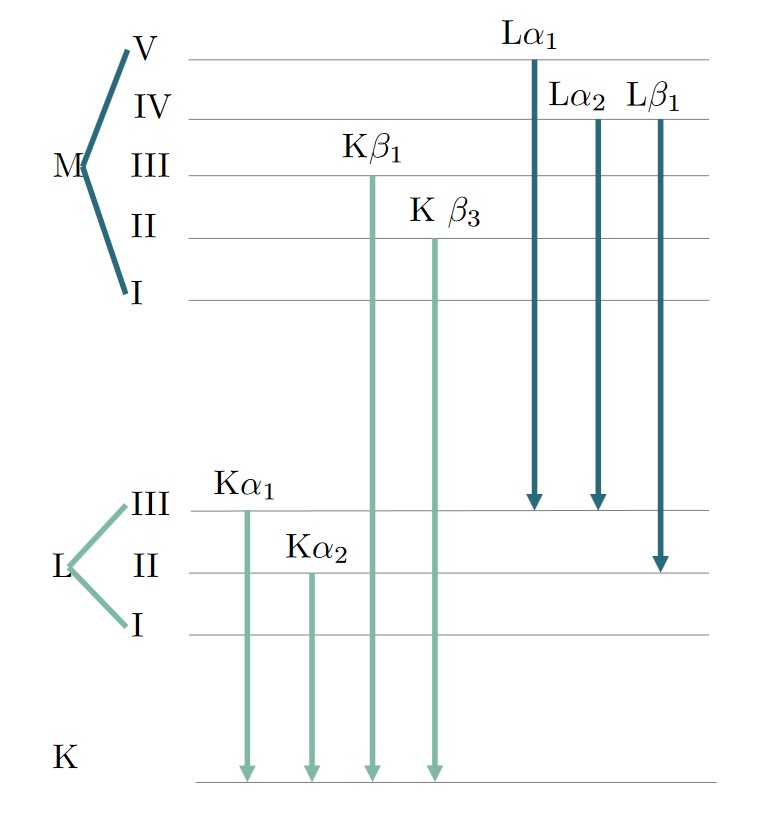
\includegraphics[width=0.5\linewidth]{figures/mari2.9-naming-lines.jpg}
    \caption{Direct copy if Maris Figure 2.9. I will make my own.}
    \label{fig:theory:theoreticalxray:naming:lines}
\end{figure}



%
%
% energy and intensity
\subsection{Energy and intensity}
\label{sec:theory:theoreticalxray:energyintensity}

% short about the energy of the characteristic X-rays
The energy of the characteristic X-ray depends on which orbital the vacancy is in, which orbital the electron is relaxed from, and the amount of protons in the core of atom A. % $\textnormal{e}^-_{3}$ 
Higher Z means higher energy of the characteristic X-ray line, because the energy difference between the relaxation orbital and the ionized orbital is larger.
Atoms with higher Z have more possible transitions, because they have more  electrons and orbitals.

%selection rules
The selection rules, which govern the allowed transitions for the formation of characteristic X-rays, are based on the Pauli exclusion principle and the spin-orbit coupling.
See \cref{fig:theory:theoreticalxray:energyintensity:quantumnumbers} for illustration of the quantum number $n$ and $l$ which are relevant for the selection rules.
Quantum number $j$ is the total angular momentum, which is the sum of the orbital angular momentum $l$ and the spin angular momentum $s$.
The selection rules in \cref{eq:theory:theoreticalxray:energyintensity:selectionrules} is for the electron which relaxes to the vacancy in the core orbital of atom A \cite[Sec. 8.2.2.2]{hollas_modern_2004}.

\begin{equation}
    \label{eq:theory:theoreticalxray:energyintensity:selectionrules}
    \Delta n \ge 1;\qquad \Delta l  = \pm 1;\qquad \Delta j = 0, \pm 1
\end{equation}

% figure from wikipedia showing n, l, j
% file: wikipedia-quantum-numbers-n-l-j.png
\begin{figure}
    \centering
    % \captionsetup{0.8\linewidth}
    % remove \colorbox to get the figure transparent again
    \colorbox{white}{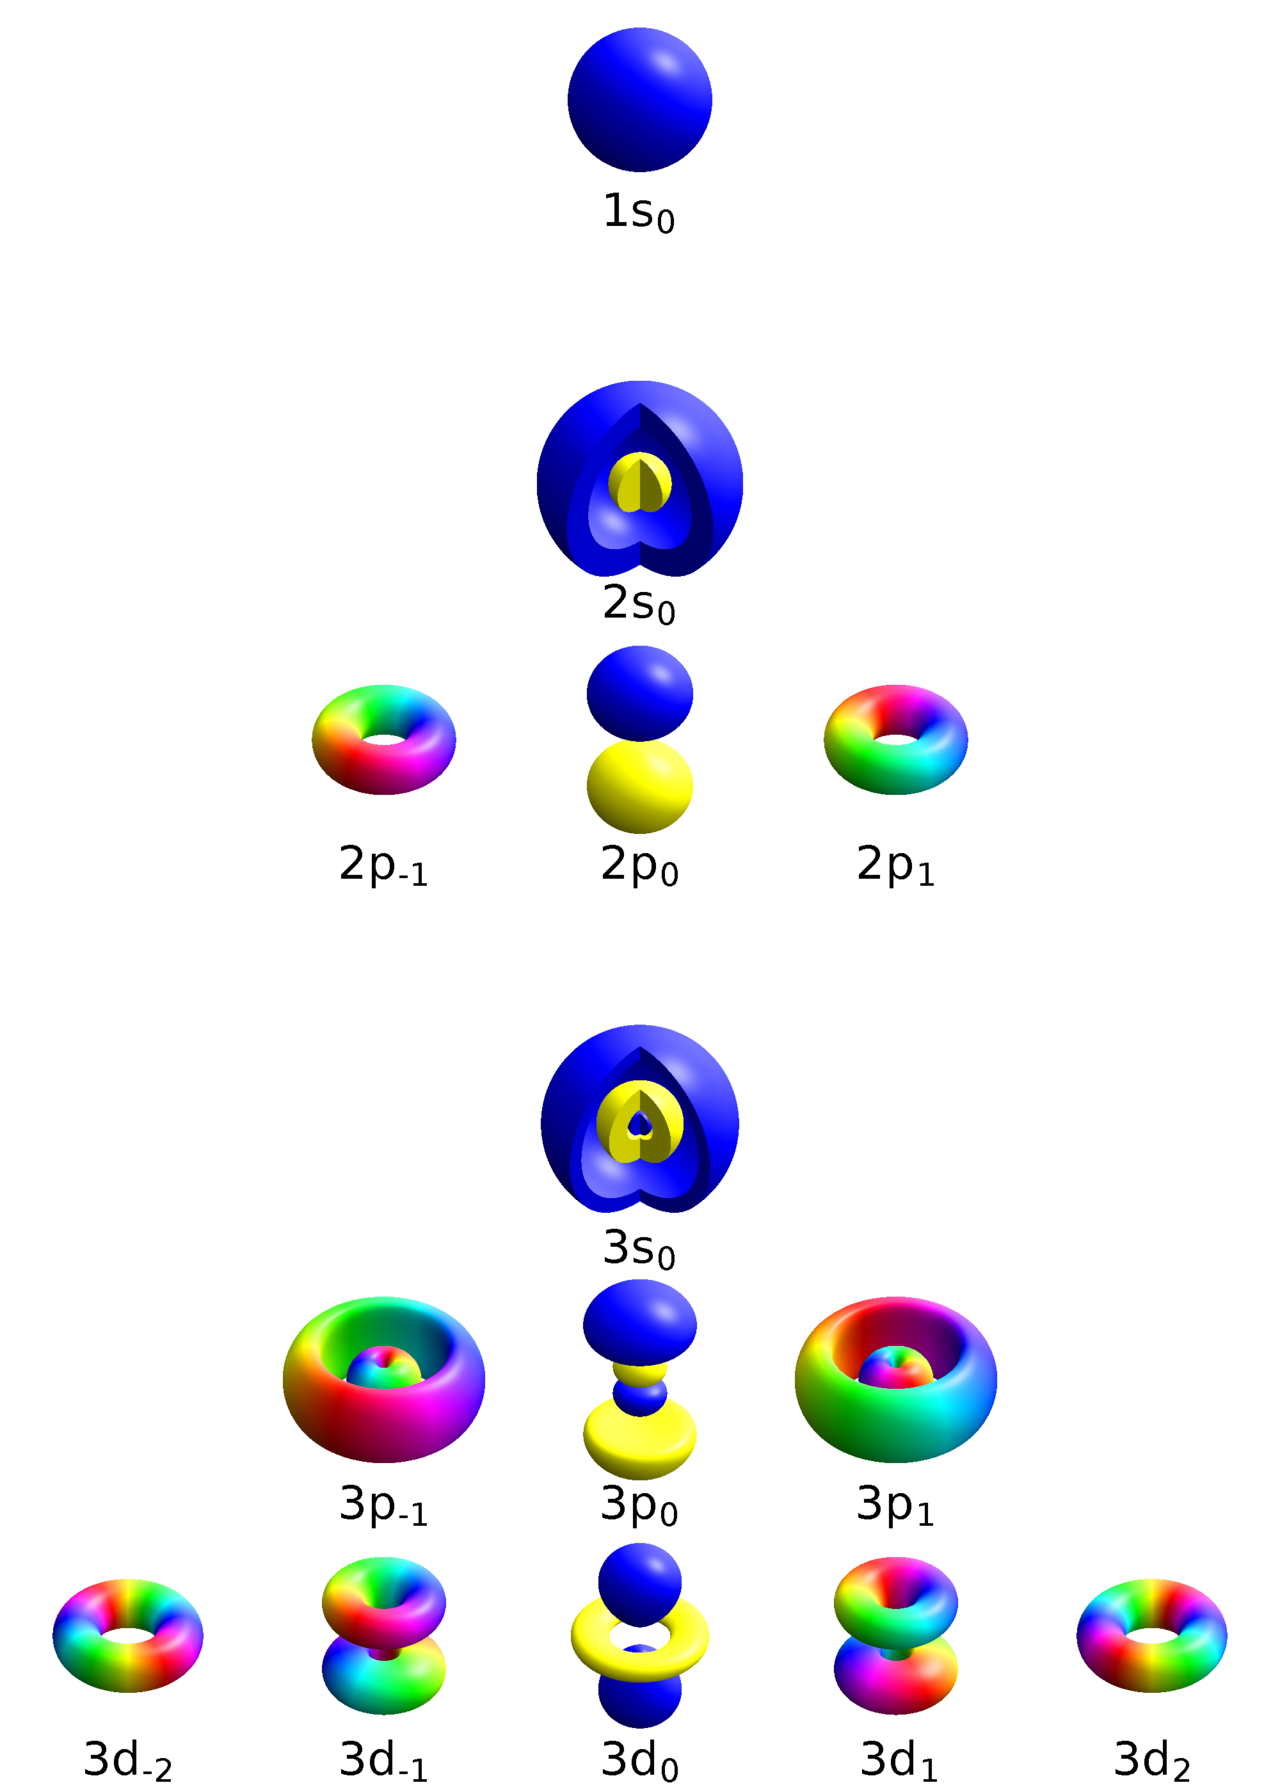
\includegraphics[width=0.5\linewidth]{figures/wikipedia-quantum-numbers-n-l-j.png}}
    \caption{
        The quantum numbers $n$, $l$, and $m$ in a hydrogen-like atom.
        The principal quantum number is shown as the block with values $n= 1, 2, 3$.
        The Azimuthal quantum number is the rows as $l = s, p, d$.
        The magnetic quantum number is the columns as $m = -2, -1, 0, 1, 2 $.
        The spin quantum number, $s$, is not geometrically dependent and thus not shown.
        The total angular momentum quantum, $l$ number is the sum of $l$ and $s$.
        The figure is copied from the article "Quantum number" on Wikipedia, made by Geek3 - Own work, Created with hydrogen 1.1, CC BY-SA 4.0, \url{https://commons.wikimedia.org/w/index.php?curid=67681892}.
    }
    \label{fig:theory:theoreticalxray:energyintensity:quantumnumbers}
\end{figure}


% intensity in theory
Even though heavy atoms like gold have more than 30 possible transitions, only a few are detectable in EDS.
Lines which are undetectable have low abundance, are too close to other lines, or are forbidden by the selection rules \cite[Ch. 4.2.3]{goldstein_scanning_2018}.
Lines which are detectable have an intensity dependent on the amount of the element in the sample, because a higher amount gives more counts in the detector.
The counts in EDS the number of X-ray photons detected in a specific energy range.
The energy range is typically around 10 eV.
In theory, the ratio of the atomic concentration between two elements are proportional to the ratio of the corresponding lines from the elements.
However, there are many factors which affect the intensity of the lines, which are covered in \cref{sec:theory:empirical}.


% figure with the whole GaAs spectrum
% figure placeholder-GaAs30kV-whole-spectrum.png
\begin{figure}
    \centering
    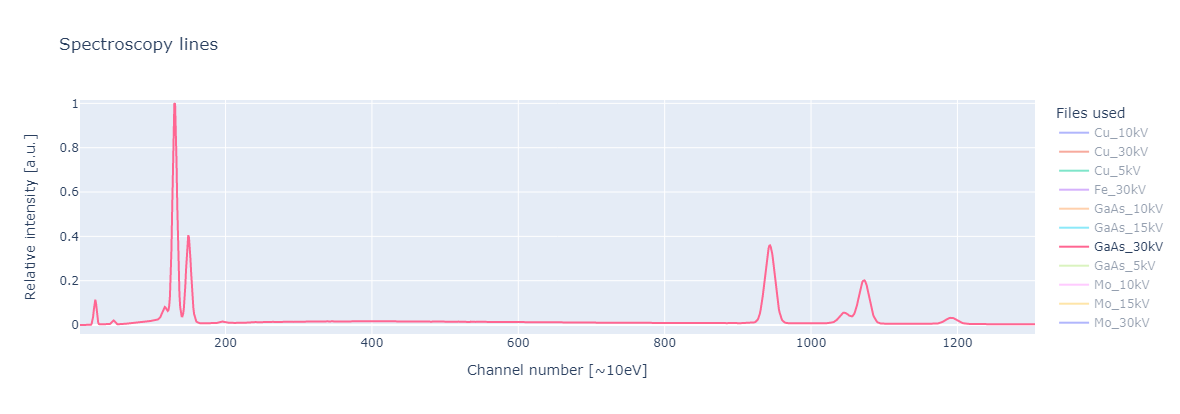
\includegraphics[width=1\linewidth]{figures/placeholder-GaAs30kV-whole-spectrum.png}
    \caption{
        The whole GaAs spectrum.
        The next two figures zoom in on different parts of this plot.
        Data from the SEM Apreo at NTNU NanoLab, 30 kV.
    }
    \label{fig:theory:GaAs30kV-whole}
\end{figure}



\begin{figure}
    \centering
    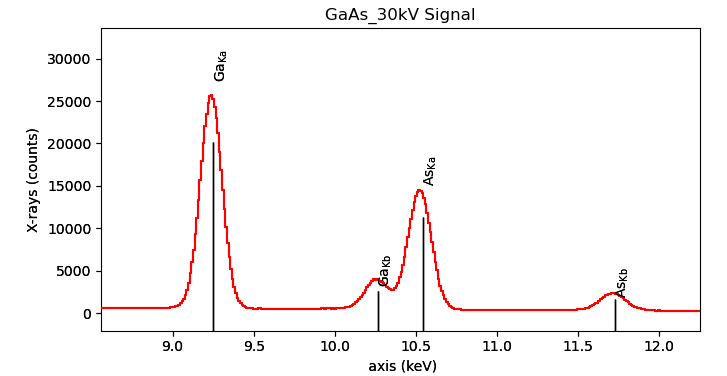
\includegraphics[width=0.9\textwidth]{figures/GaAs30kV-8-12keV.png}
    \caption{
        Plot produced by HyperSpy of the X-ray lines in GaAs from 8 to 12.5 keV.
        The theoretical lines are marked with black lines, but in reality the lines become peaks with Gaussian shapes.
        The height of the black lines are empirically estimated and are available in HyperSpy.
        Notice also how the center of the peak and the black line are slightly right shifted, which can be solved by calibrating the energy scale, see \cref{sec:theory:calibration}.
        Data from the SEM Apreo at NTNU NanoLab, 30kV.
    }
    \label{fig:theory:GaAs30keV-8-12-keV}
\end{figure}

\begin{figure}
    \centering
    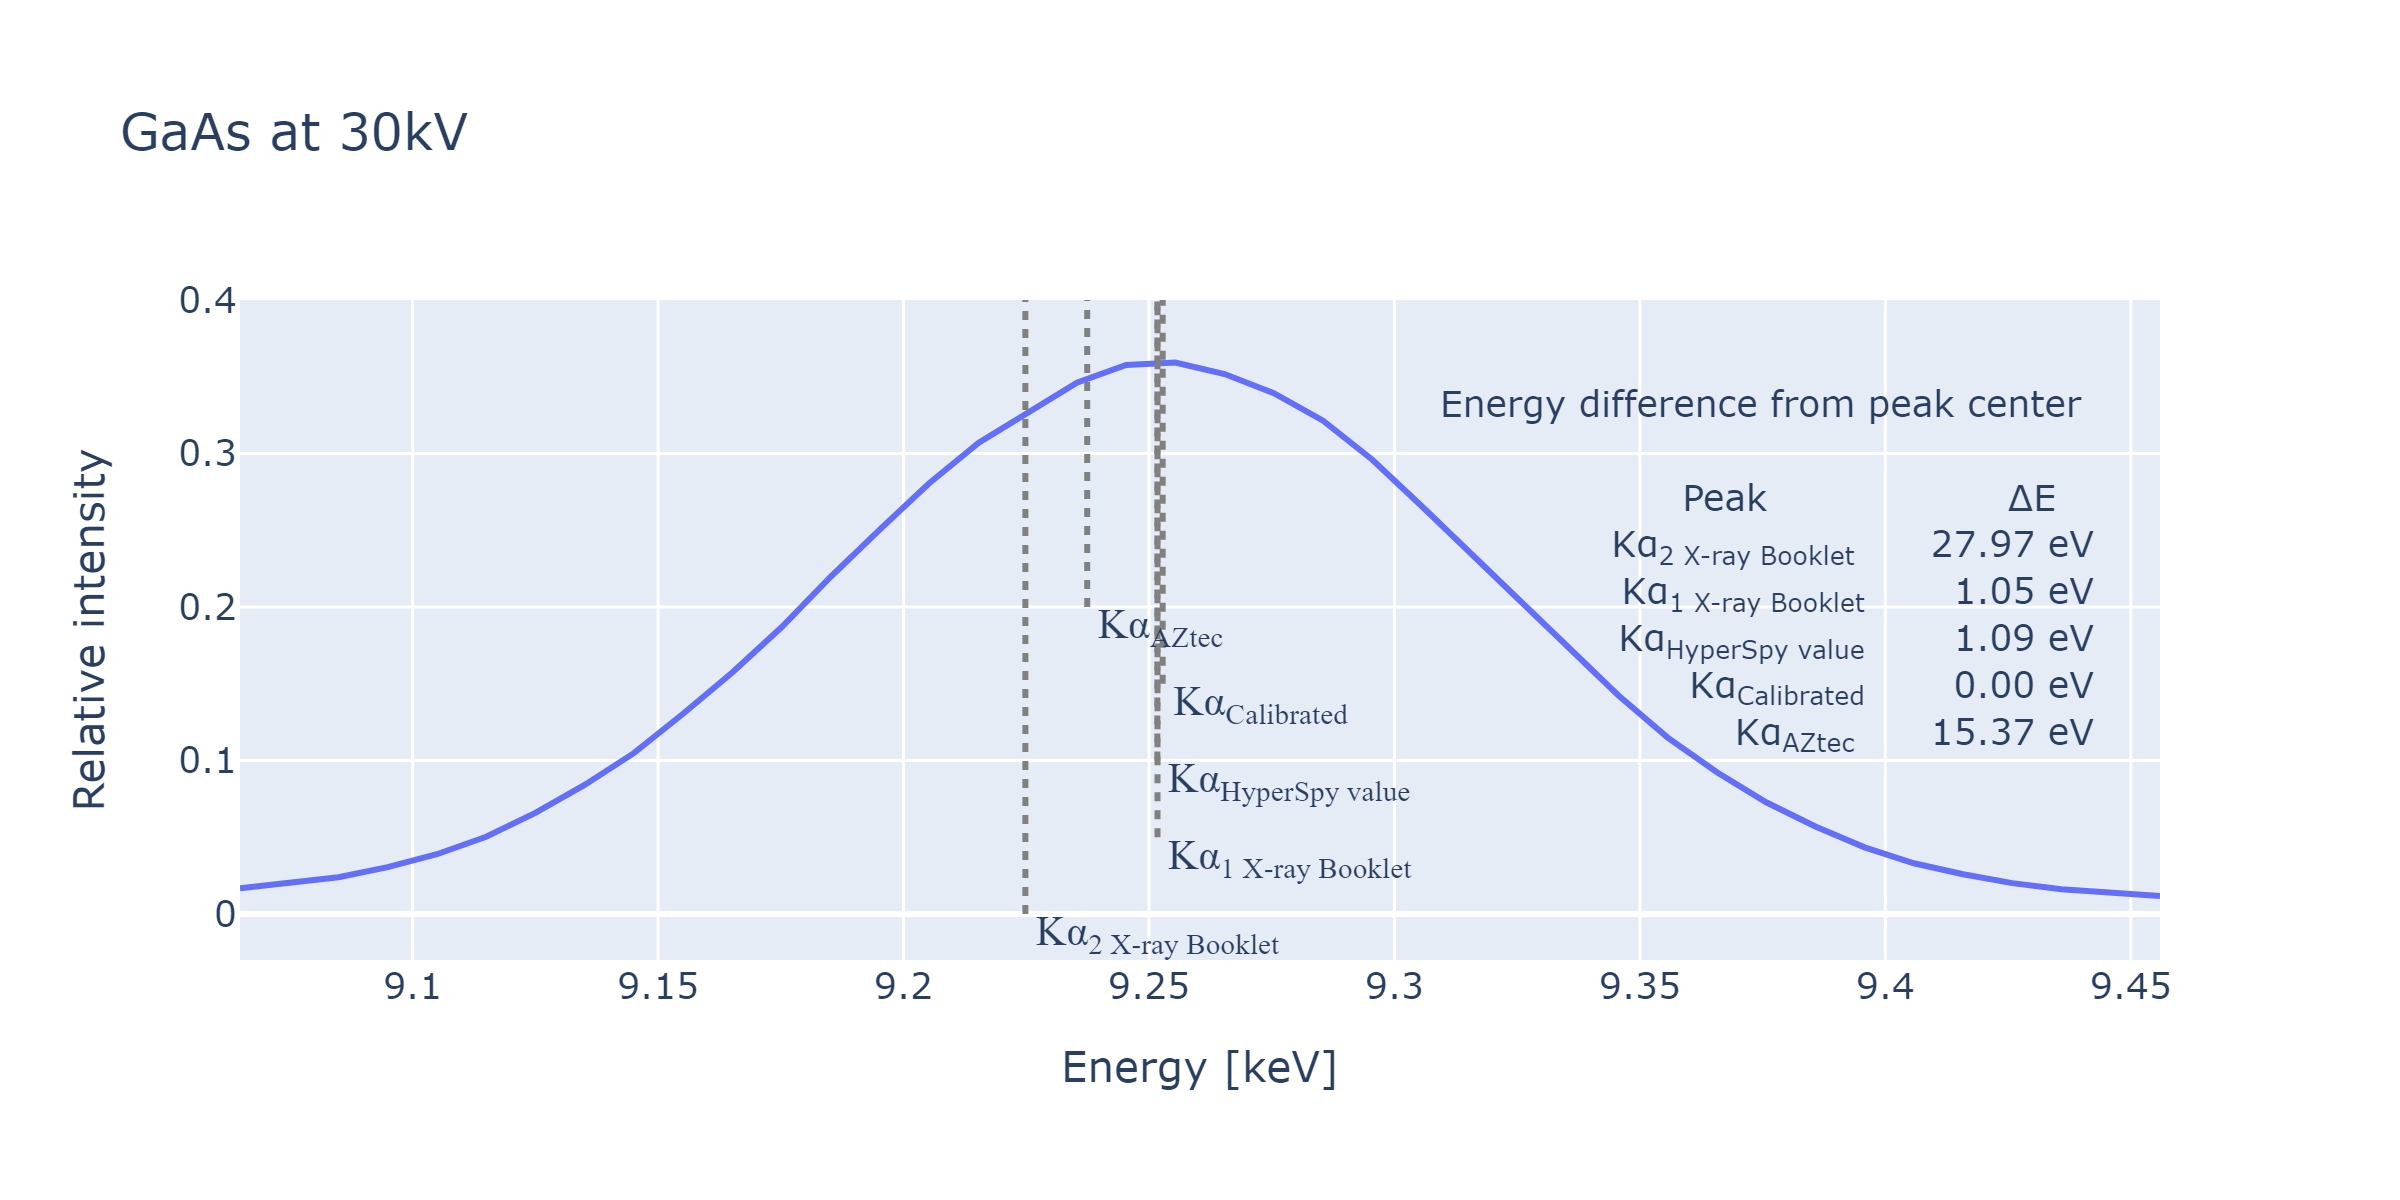
\includegraphics[width=0.9\textwidth]{figures/GaAs30kV-Ga-K-lines.png}
    \caption{
        The theoretical lines K$\alpha_1 = 9.25174$ and K$\alpha_2 = 9.22482$ from the X-ray booklet with K$\alpha = 9.251$ from HyperSpy and the fitted peak K$\alpha$.
        The spectrum is calibrated to Ga $L\alpha$ and As K$\alpha$, where the energy of the peaks is taken from HyperSpy.
        HyperSpy gives Ga K$\alpha$ almost directly on top of the theoretical K$\alpha_1$.
        This figure show that the lines which are separated with small energy differences are so close that they make one single peak in the EDS spectrum.
        Data from the SEM Apreo at NTNU NanoLab, 30kV.
        \ton{This is more results than theory I would say. But I do remember you saying something about having this in the theory section.}
    }
    \label{fig:theory:GaAs30keV-K-lines}
\end{figure}

% theoretical values of the lines
% include the table in table/Ga-lines.tex
% table listing the Ga lines, both from Hyperspy and from the X-ray booklet

\begin{table}[tbp]
    \centering
    \caption{
        Ga lines from HyperSpy cite ?? and X-ray booklet \cite{thompson_x-ray_2004}.
        ** HyperSpy operates with a single line for each K and L shell, but the X-ray booklet lists two lines for each shell.
        * HyperSpy lists Ln, Ll and L$\beta_3$ as separate lines, but I am not sure what they correspond to in the X-ray booklet.
        TODO: Figure out this.
    }
    \label{tab:theory:Ga-lines}
    \begin{tabular}{llll}
                       & X-ray booklet & HyperSpy     & HyperSpy \\
                       & Energy [keV]  & Energy [keV] & Weight   \\
        \hline
        K$ \alpha_1$   & 9.25174       & 9.2517       & 1.0      \\
        K$ \alpha_2$** & 9.22482       &              &          \\
        K$ \beta_1$    & 10.2642       & 10.2642      & 0.1287   \\
        L$ \alpha_1$   & 1.09792       & 1.098        & 1.0      \\
        L$ \alpha_2$** & 1.09792       &              &          \\
        L$ \beta_1$    & 1.1248        & 1.1249       & 0.16704  \\
        L$n$*          &               & 0.9843       & 0.02509  \\
        L$l$*          &               & 0.0544       & 0.9573   \\
        L$b_3$*        &               & 0.0461       & 1.1948
    \end{tabular}

\end{table}




%
%
%
%
\section{Empirical view on characteristic X-rays}
\label{sec:theory:empirical}
On top of the theoretical physics there are many experimental processes affecting both the creation and the detection of characteristic X-rays.
The scientific community uses an empirically influenced approach in EDS analysis.
This approach includes empirical equations to deal with the imperfect beam, scattering in the chamber, secondary scattering (?), imperfect detectors, \dots

\ton{What do I do with the thin film assumptions? How do I mention it?}

%
%
%   - from lines to peaks
%     - broadening of line to peaks
%     - peak shape, gaussian
\subsection{From lines to peaks}
\label{sec:theory:empirical:peaks}
A striking difference between the theoretical and the empirical view is that the lines are not lines, but peaks with a varying width.
This is illustrated both in \cref{fig:theory:GaAs30keV-8-12-keV} and in \cref{fig:theory:GaAs30keV-K-lines}, where we see that the two K$\alpha$ lines of Ga is merged into one broad peak.
The peaks in the EDS spectrums have a Gaussian shape, which is a result of the broadening of the lines.
The broadening of the lines is due to \dots \ton{What is the cause of the broadening? And why is it Gaussian?}. % count statistics!
\cref{fig:theory:GaAs30kV-whole} shows that lower energy lines are narrower than higher energy lines.
This increase in broadening with higher energy is due to \dots \ton{What is the cause of the broadening with higher E again?}

\brynjar{Write more here.}
A Gaussian peak is a curve defined by the following equation:

\begin{equation}
    \label{eq:theory:empirical:gaussian}
    g(x) = \frac{1}{\sigma \sqrt{2\pi}} exp({-\frac{(x-\mu)^2}{2\sigma^2}})
\end{equation}

In the equation $\mu$ is the center of the peak, $\sigma$ is the standard deviation, and $x$ is the energy.
When doing peak fitting, the first term is treated as the amplitude and is a parameter which is fitted, i.e. $1/\sigma\sqrt{2\pi}$ is swapped with a parameter $A$.
$\mu$ and $\sigma$ are also fitted parameters, where $\mu$ is the center of the peak and $\sigma$ is the width of the peak.
$x$ is the energy, i.e. the x-axis in the EDS spectrum.

The width of the peak is a measure of the broadening of the line, and is usually given as the FWHM in EDS analysis. The FWHM is connected to the standard deviation of the Gaussian distribution, which is given by \cref{eq:theory:empirical:gaussian}.
The FWHM can be calculated from the standard deviation, $\sigma$, with:

% Eq FWHM
\begin{equation}
    \label{eq:theory:empirical:peaks:FWHM}
    \textnormal{FWHM} = {\sigma}{2\sqrt{2\ln(2)}}
\end{equation}


%
% 
%   - intensities
%     - weight of a line intro
%     - fluorescent yield approx
%     - empirical weights in HyperSpy,
%     - k-factor
%     - k-ratio
\subsection{Intensity}
\label{sec:theory:empirical:intensity}

% intensity in reality
% put this in the empirical section, just say that it is lower for low energy because of many reasons (absorption, efficiency). Same reason than background is lower for low energy. 

% remove?
% After the first relaxation there is also an avalanche of following relaxation events to the new hole in the relaxed orbital.
% All but the first relaxation are too low in energy to be detected as characteristic X-rays in EDS.

% weight of a line
The intensity, or weight, of a line is dependent on multiple empirical and physical factors.
This subsection will briefly cover fluorescent yield, critical ionization energy, and empirical weights in HyperSpy.
In practice, the weight of the lines are included as a part of the k-factors or k-ratios, which are presented in \cref{sec:theory:empirical:kfactors}.
Only the strongest lines are listed in the X-ray booklet, where the theoretical values of the characteristic X-ray lines are listed.
The list include: K$\alpha_1$, K$\alpha_2$, K$\beta_2$, L$\alpha_1$, L$\alpha_2$, L$\beta_1$, L$\beta_2$, L$\gamma_1$, M$\alpha_1$ \cite{thompson_x-ray_2004}.
HyperSpy operates with a different list of lines, which might be more empirically influenced.
The lines for Ga is for instance:
The lines for Mo is:
The lines for a heavy element like Sb(?) is:
\brynjar{Fyll inn disse.}


%%%%% TODO %%%%%
% write about the Mo Ll and Mo L$\gamma$3 peaks in the teory section.

% HYperSpy and X-ray booklet are not the same. HS more empirical?













% fluorescent yield
\brynjar{This info about fluorescent yield is interesting, but will I actually use it?}
The fluorescent yield $\omega$ is non-linearly dependent on $Z$.
Figure (4.3)  in Goldstein \cite{goldstein_scanning_2018} \ton{Reproduce the figure? Would take like 2h to use the Crawford data properly I guess} shows the fluorescent yield for the first 90 elements (which is based on Crawford 2011).
For K- and L-shell fluorescent yield, $\omega$ is strictly increasing.
For M-shell fluorescent yield, $\omega$ is strictly increasing till around $Z=80$, and then it starts to decrease.
The figure also show that for the same element $\omega_{\textnormal{K}}  > \omega_{\textnormal{L}} > \omega_{\textnormal{M}}$ \brynjar{But L-peaks are higher in the spectra. Explain this in the discussion?}.
When dealing with thin samples, the fluorescent yield can be approximated by an empirical formula based on tin.
The formula is given in \cref{eq:empirical:fluorescentyieldapprox}, where $a=10^6$ for K-shell. \brynjar{What is it for L and M? Also, is it really relevant here?}
The two key takeaways from this formula is that $\omega$ is dependent on $Z$, but kinda similar for close elements like Ga $Z = 31$ and As $Z = 33$.

\brynjar{Find the source for this formula. Ton said it is from Williams and Carter. Is it valid for bulk? The K-shell have the same shape as Figure 4.3 in Goldstein.}

\ton{I'm not sure if I will actually use this formula, should I just remove it? And I don't get how this formula just becomes a part of the k-factor. Except from the key takeaways mention above.}

\begin{equation}
    \label{eq:empirical:fluorescentyieldapprox}
    \omega = \frac{Z^4}{a + Z^4}
\end{equation}

% critical ionization energy
The critical ionization energy, $E_\textnormal{C}$, is the energy the incident beam need to ionize a core electron in an atom.
If the energy of the incident beam is lower than $E_\textnormal{C}$, the core electron is not ionized and no peak can be detected.
The critical ionization energy is dependent on the atomic number, $Z$, of the atom.
Higher $Z$ means higher $E_\textnormal{C}$, because the core electrons are bound stronger to the nucleus.
When the incident beam has an energy higher than $E_\textnormal{C}$ and continues to increase, the amount of ionization is not constant and not linear.
The amount of ionization with varying energy above $E_\textnormal{C}$ is dependent on the ionization cross section and the overvoltage, which again are dependent on what shell the ionization happens in.
The solution to this is empirically estimations and using k-factors where all factors like this is either cancelled out or included in the k-factor correction.

% Ionization cross section and overvoltage
\ton{Is this good enough? If not, what do I write about the ionization cross section and overvoltage? What Mari wrote is for thin samples, I think. Why include it if I'm not going to use any equations about the ionization cross section or overvoltage? You said something about just write that intensity it is lower for low energy because of many reasons (absorption, efficiency), with the same reason that background is lower for low energy. But I kinda need to explain some reasons to use them in the discussion. Another question: in the k-factor all these other factors fall out, so EDS-people does not use these equations. Am I wrong?}

% empirical weights in HyperSpy
HyperSpy have an integrated list of the characteristic X-rays, with both the energy and the weight of the lines.
\brynjar{I guess the weights are empirically estimated, but I have not found any information about how they are estimated. In addition: I'm not sure if HyperSpy adjust the line height to the spectrum, or if it knows that Ga K$\alpha$ are higher than As K$\alpha$ as in \cref{fig:theory:GaAs30keV-8-12-keV}.}
Goldstein uses different intensity weights for isolated atoms, thin foils and bulk samples \cite[Ch. 4.2.6]{goldstein_scanning_2018}, and all are dependent on the atomic number and ionized shell.
One could venture down the rabbit hole of finding the theoretical weights for different lines, but that will not be done in this thesis.
Examples of the weights from HyperSpy are given in \cref{tab:theory:Ga-lines}.
\ton{OK?}


%
% 
% k-factors
% k-ratios
\subsection{Cliff-Lorimer and the k-factors}
\label{sec:theory:empirical:kfactors}
About the k-factors, and perhaps the k-ratios as well.

Cliff-Lorimer is page 23 in Skomedal.

Explain the equations and where they come from.

Castaings model:

\begin{equation}
    \frac{C_\textnormal{i}}{C_\textnormal{(i)}} = K \frac{I_\textnormal{i}}{I_\textnormal{(i)}}
\end{equation}

Cliff and Lorimer took it further and swapped the standard for the ratios of intensities from two elements measured in the same spectrum:

\begin{equation}
    \frac{C_\textnormal{a}}{C_\textnormal{b}} = \frac{k_\textnormal{a} I_\textnormal{a}}{k_\textnormal{b} I_\textnormal{b}} = k_\textnormal{ab}  \frac{I_\textnormal{a}}{I_\textnormal{b}}
\end{equation}




% %   - energy issues
% %     - overvoltage (deviations from q-mec, something in my notes)
% \subsection{Energy}
% \label{sec:theory:empirical:energy}
% \brynjar{Do I have something here? Can't recall what I wanted to include, which is not covered in other subsections.}



%   - the detection system
%     - detector efficiency
%     - detector resolution
%     - dead time
%     - angle/placement of detector
%     - beam issues
%     - stray: secondary excitations in the sample
%     - Si stray
%     - holder / chamber stray detection
\subsection{Detection system}
\label{sec:theory:empirical:detectionsystem}
Detector efficiency, detector resolution, dead time, angle/placement of detector, beam issues, stray: secondary excitations in the sample, Si stray, holder / chamber stray detection.

\subsection{Sample thickness}
\label{sec:theory:empirical:samplethickness}
Thin vs bulk samples.
%   - thin and bulk samples



%
%
\subsection{Bremsstrahlung - the background radiation}
\label{sec:theory:empirical:background}
Why linear and why sixth order polynomial. Which are better.
\brynjar{I might use background removal as some results, but I'm not sure. That would be comparing the different methods, and looking at smoothing of the data before removing the background.}

\brynjar{TODO: Include a illustration of background. } % label fig:theory:background_illustration

%
%
% calibration of the spectrum
\section{Calibration of the spectrum}
\label{sec:theory:calibration}
% my notebook

% equation dispersion = e2 - e1 / c2 - c1

$E_1$ and $E_2$ is the energy of the two characteristic X-rays, and $c_1$ and $c_2$ is the channel number of the two characteristic X-rays.

\begin{equation}
    \label{eq:theory:calibration:dispersion}
    \textnormal{Dispersion} = \frac{E_2 - E_1}{C_2 - C_1}
\end{equation}

Get as little extrapolation as possible by selecting the longest possible distance between the two characteristic X-rays, while still using peaks with good signal-to-noise ratio.
\brynjar{Quantify signal-to-noise ratio?}
Assume calibration on one spectrum and use it on all spectra for the same instrument.


Zero-offset in channels is:
\begin{equation}
    \label{eq:theory:calibration:offset}
    \textnormal{Zero-offset in channels} = C_1 - E_1 \cdot \textnormal{Dispersion}
\end{equation}

% dispersion
% zero-offset


\section{SEM}
\label{sec:theory:sem}


- how (e-beam, vacuum, ...)
- hardware (scanning coils, astigmatism)
- imaging (contrast, SE, BSE)


% Data processing (hvis jeg kommer dit)
% - ML, støybehandling
% - future work?
% - Ton er skeptisk



% PCA, ICA ???????? Gjøre noe faktisk statistikk?

